\section{GIGADuck}
\subsection{Data selection}
The  radio baseline  we  observe is  a  results of  several known  and
unknown effects. A daily modulation is due to the temperature and will
be corrected for in  section~\ref{sec:tempdep}.  Humidity can affect a
lot the baseline, but the  parameterization is more difficult. We also
notice some large change of the  baseline that are likely to be due to
storm.  We  present in this  section the cut  we operate to  clean the
data and keep  the period when the baseline is  mainly affected by the
temperature.\\In principle  we could make cuts on  humidity value, but
the  monitoring information  is not  always present.   We  operate the
selection only  the shape  of the radio  baseline and select  the days
when  the variations  are smooth.   The figure~\ref{fig:selectedpopey}
shows  the day  selected for  the  station Popey.   For instance,  the
period around  the 25th of March  was certainly a period  of rain, and
the  baseline of  Chape and  Popey is  affected, thus  this  period is
removed  from  the  dataset.   (The  date are  also  reported  in  the
appendix)
%% \begin{figure}[!ht]
%%   \centering
%%   \hspace*{-3ex}
%%   \subfigure{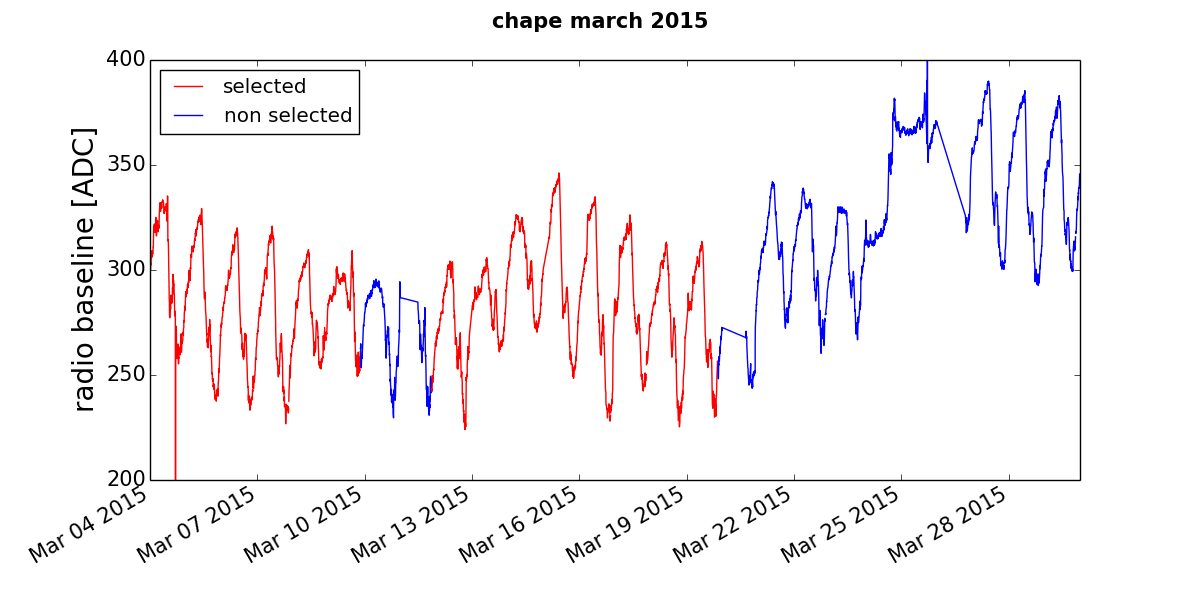
\includegraphics[width=0.49\linewidth]{chapemarch2015.png}}
%%   \subfigure{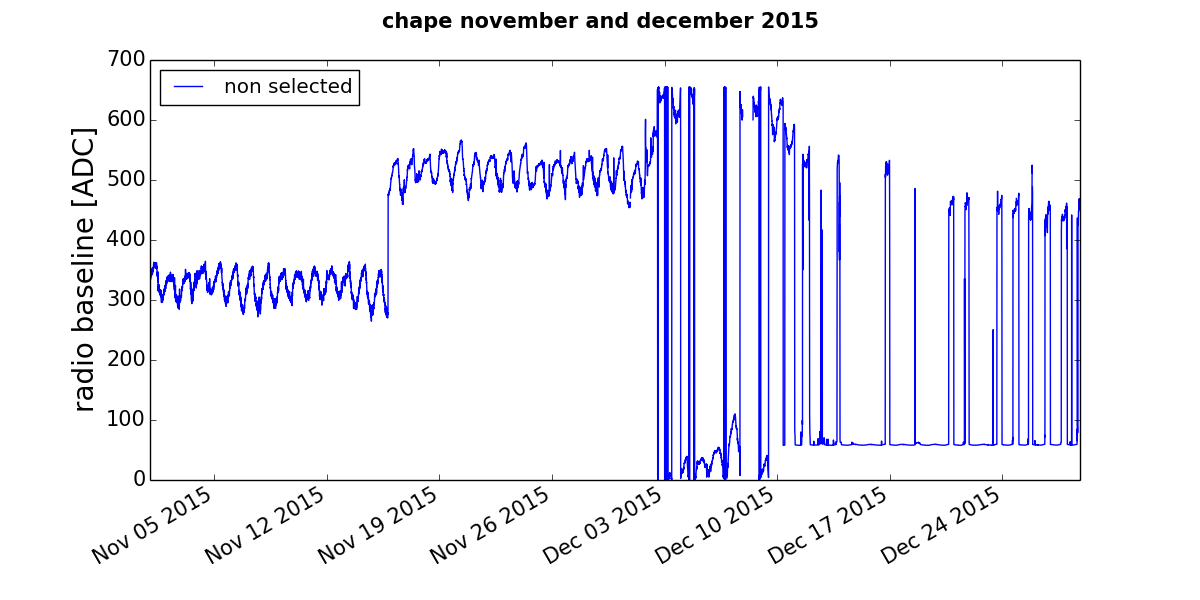
\includegraphics[width=0.49\linewidth]{chapenovdec2015.png}}\\
%%   \subfigure{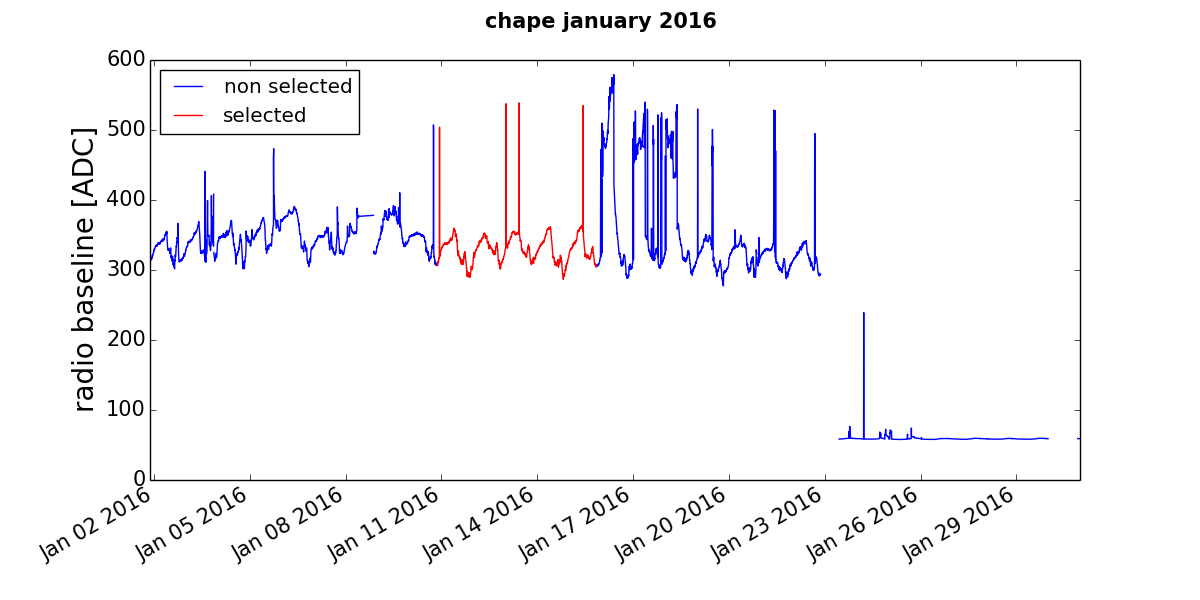
\includegraphics[width=0.49\linewidth]{chapejan2016.png}}
%%   \subfigure{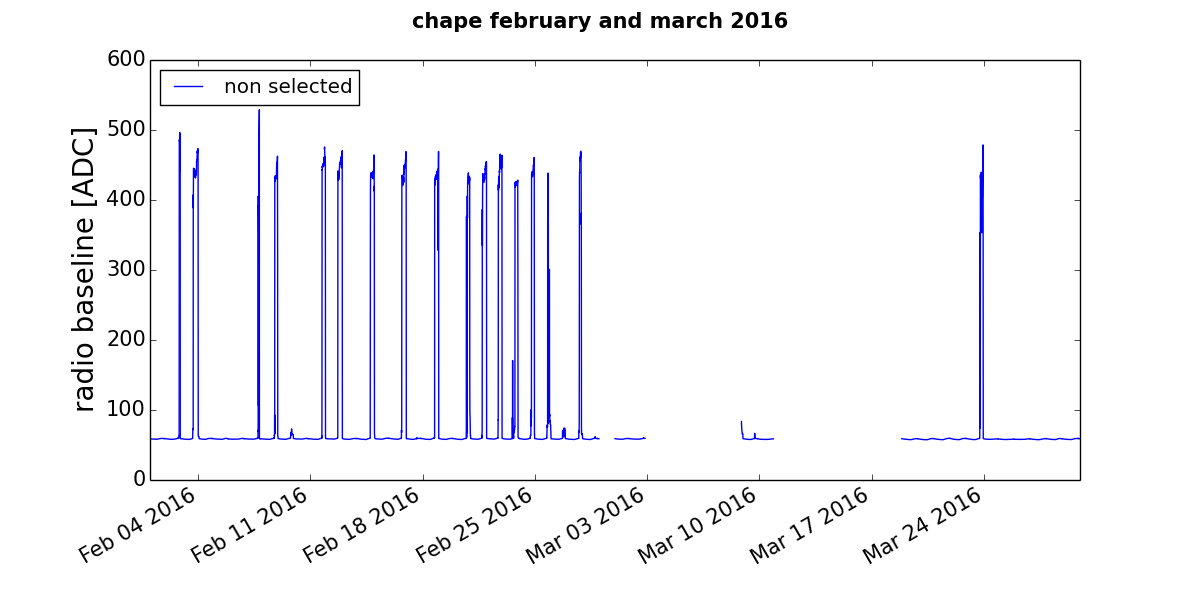
\includegraphics[width=0.49\linewidth]{chapefebmarch2016.png}}
%%   \caption{Radio baseline for four different periods for Chape station
%%     (id=384). In  red are the periods  kept for the  sun transit analysis
%%     based on the shape.}
%%   \label{fig:selectedchape}
%% \end{figure}

\begin{figure}[!ht]
  \centering
  \hspace*{-3ex}
  \subfigure{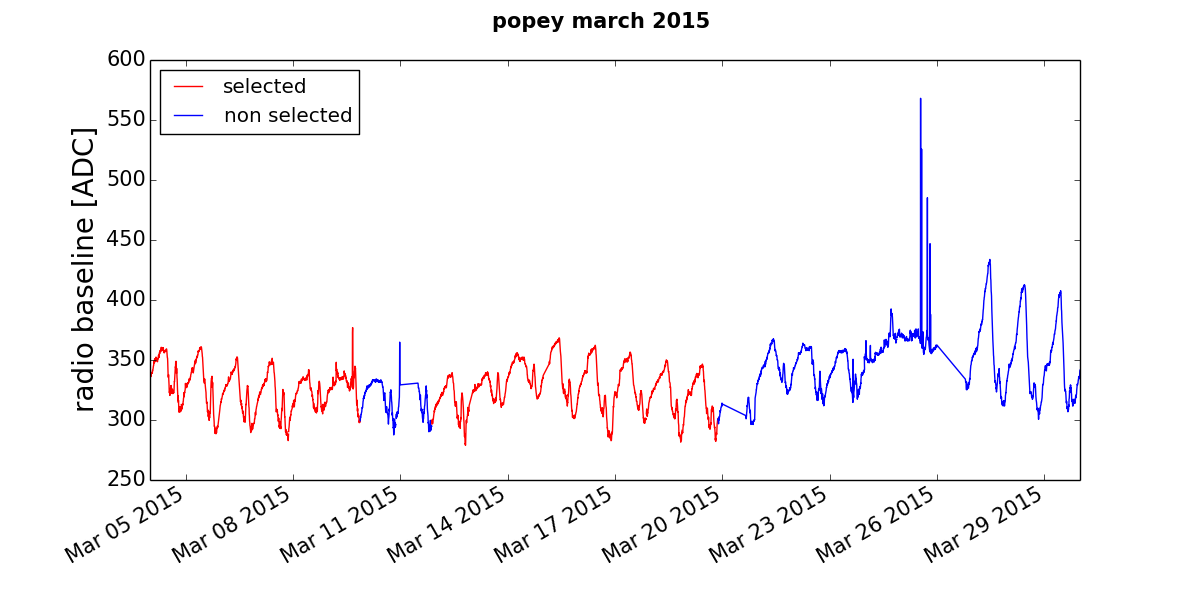
\includegraphics[width=0.49\linewidth]{popeymarch2015.png}}
  \subfigure{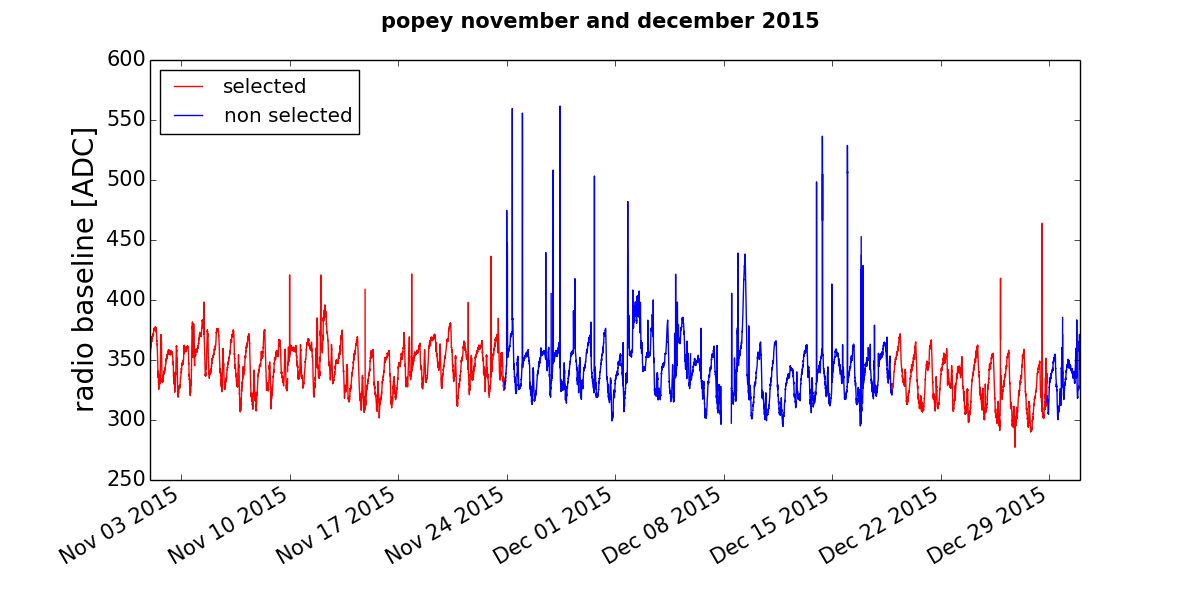
\includegraphics[width=0.49\linewidth]{popeynovdec2015.png}}\\
  \subfigure{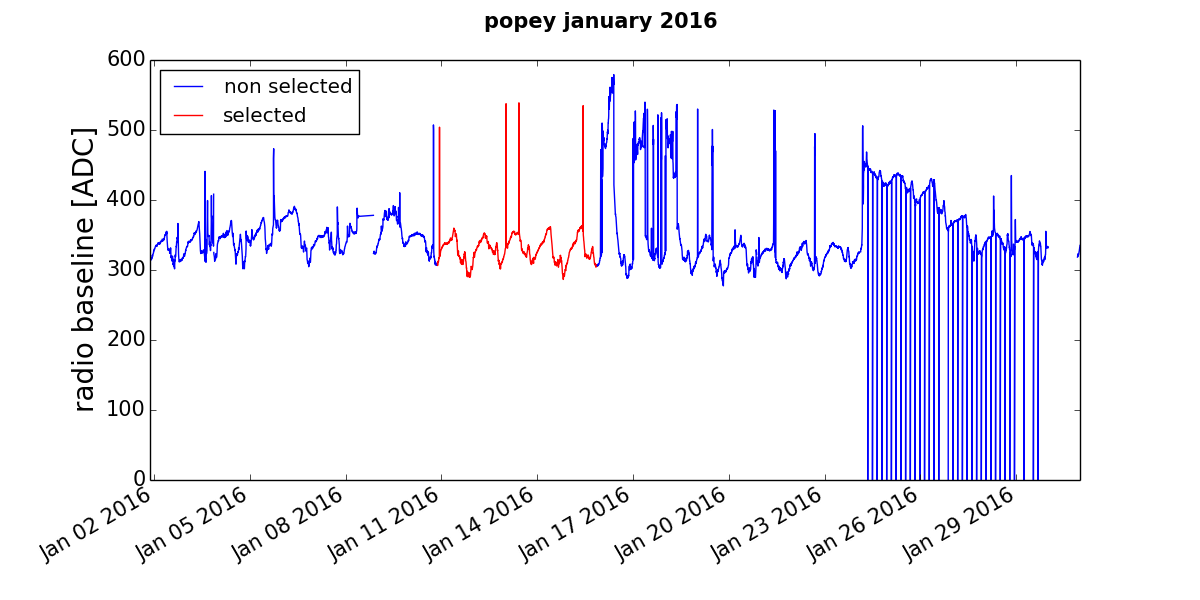
\includegraphics[width=0.49\linewidth]{popeyjan2016.png}}
  \subfigure{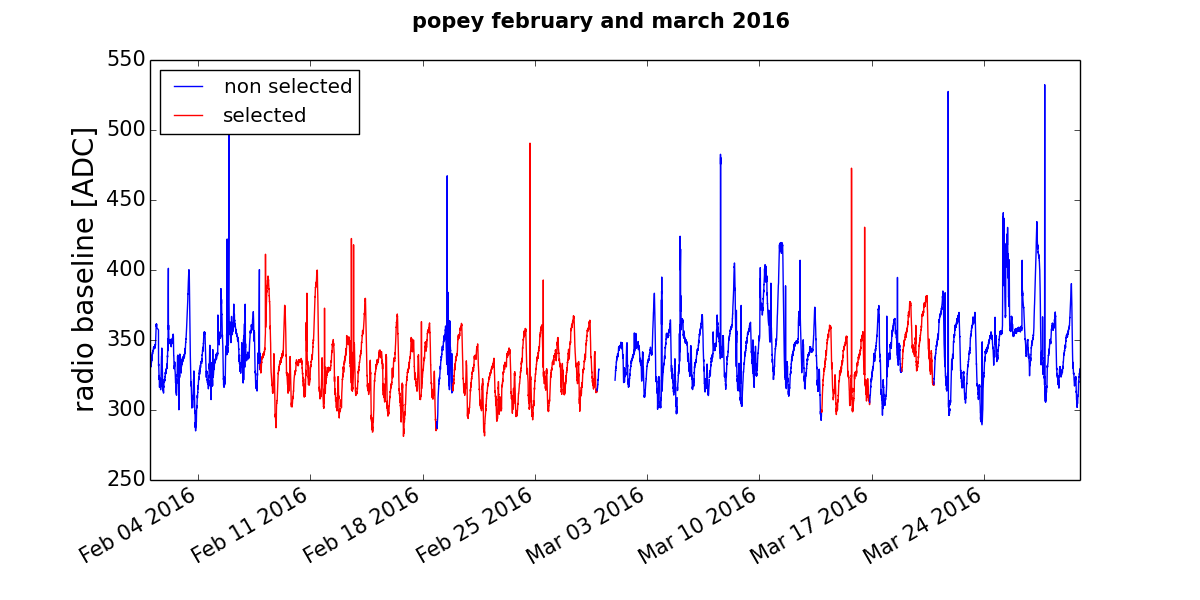
\includegraphics[width=0.49\linewidth]{popeyfebmarch2016.png}} 
  \caption{Radio baseline for four different periods for Popey station
    (id=385). In  red are the periods  kept for the  sun transit analysis
    based on the shape.}
 \label{fig:selectedpopey}
\end{figure}

\newpage
\subsection{Temperature dependence}
\label{sec:tempdep}  
The next step  is to correct from the effect  of temperature. First of
all we remove the time of the  day when the sun is expected (this time
depends on  the station because they point  toward different azimuth).
The  raw  plot  of  the  baseline  vs  temperature  is  shown  on  the
figure~\ref{fig:blvstempraw}.   For  Chape  we  notice  two  separated
populations. This is due to the  fact that we have sometimes a jump of
the baseline. To circumvent this  effect, we reference our data to the
daily average (see Figure~\ref{fig:blvstempmeansub}).  We parameterize
only the  variation of  the radio baseline  with the variation  of the
temperature:
\begin{itemize}
\item Chape: $\rm ADC - <ADC> = -2.93 (T - <T>) $
\item Popey: $\rm ADC - <ADC> = -3.67 (T - <T>) $ 
%\item Chape:  $\rm ADC - <ADC> = -2.93 (T - <T>)  -2.38\cdot10^{-5}$
%\item Popey: $\rm ADC - <ADC> = -3.67 (T - <T>)  -3.58\cdot10^{-6}$ 
\end{itemize}


\begin{figure}[!ht]
  \centering
  \hspace*{-3ex}
  \subfigure{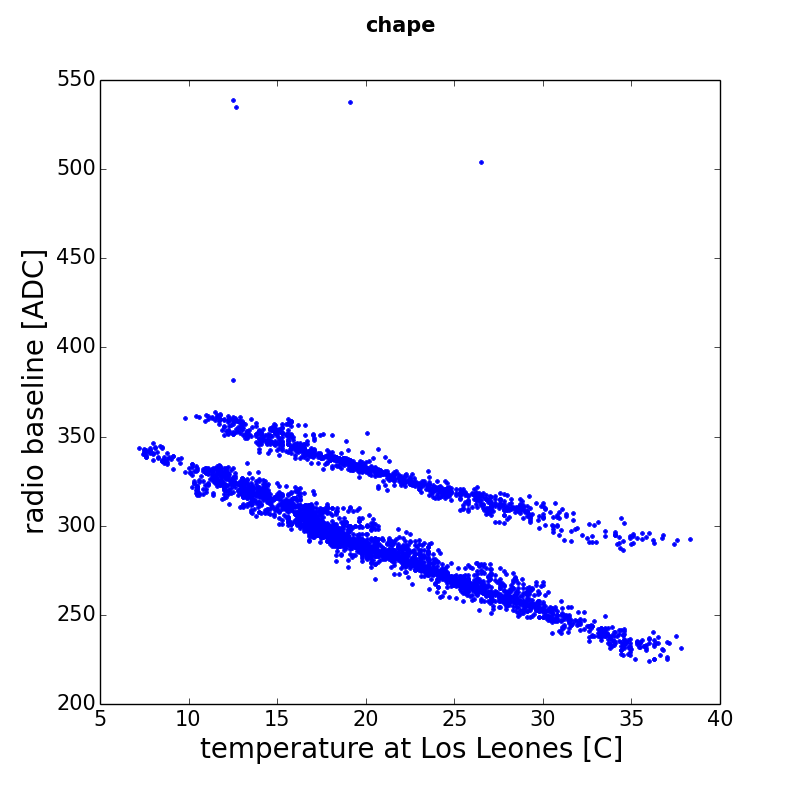
\includegraphics[width=0.49\linewidth]{chapeblvstempraw.png}}
  \subfigure{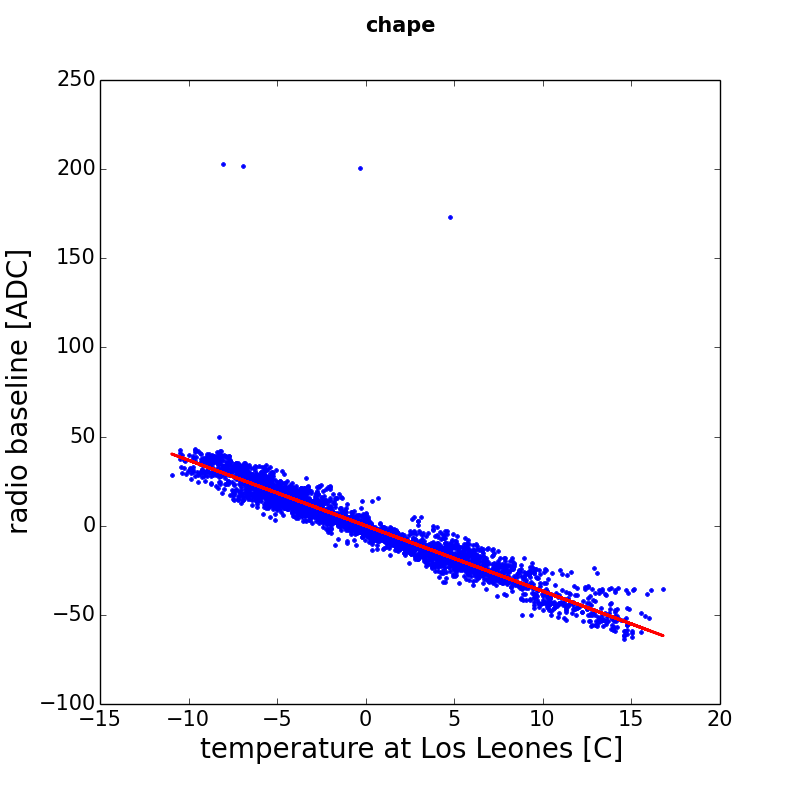
\includegraphics[width=0.49\linewidth]{chapeblvstempmeansub.png}}
  \caption{Selected period in red for Popey}
 \label{fig:blvstempraw}
\end{figure}

%% \begin{figure}[!ht]
%%   \centering
%%   \hspace*{-3ex}
%%   \subfigure{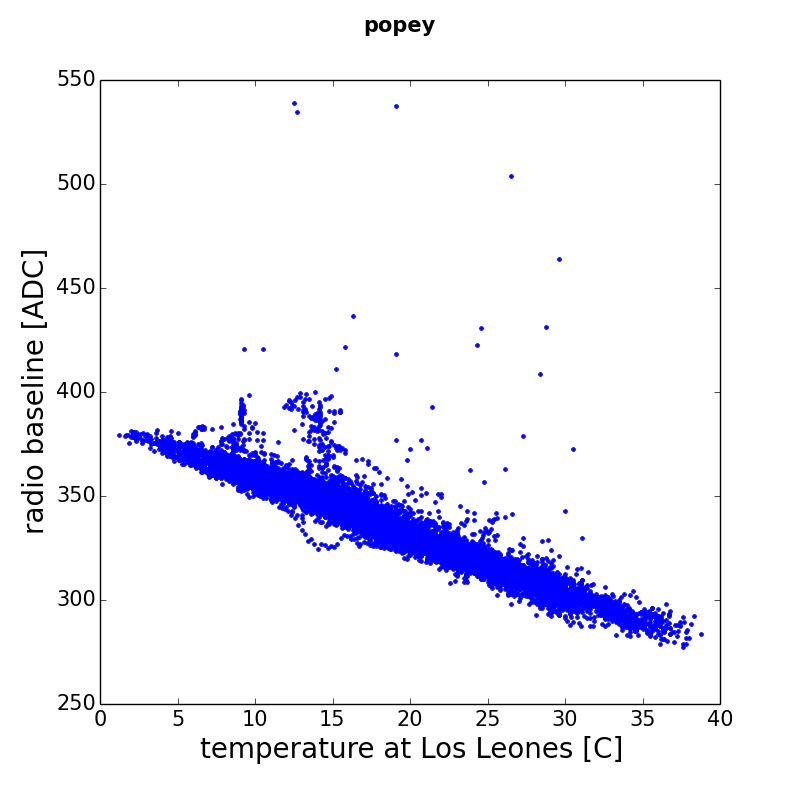
\includegraphics[width=0.49\linewidth]{popeyblvstempraw.png}}
%%   \subfigure{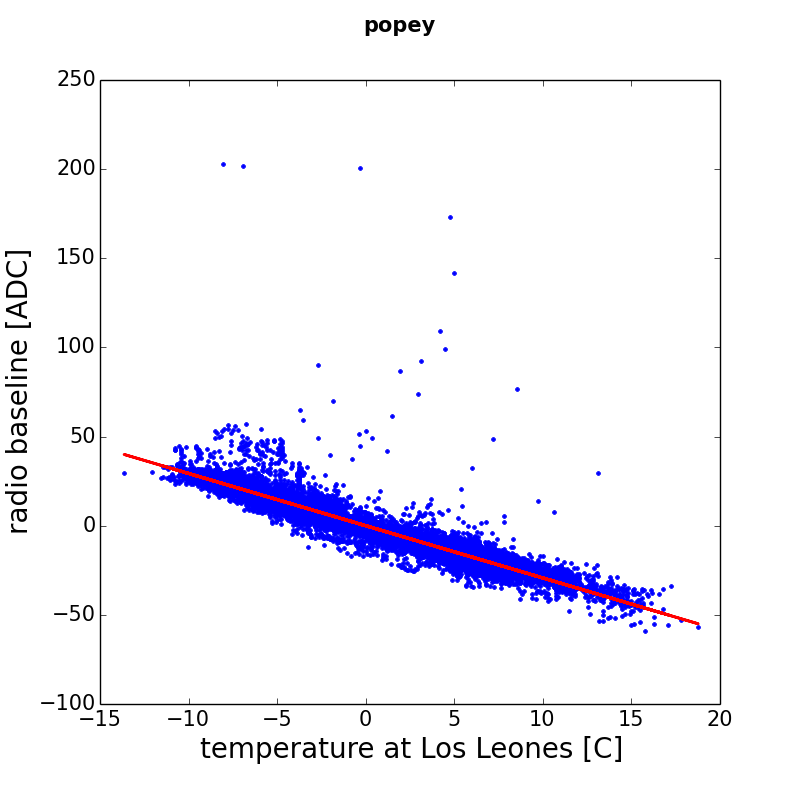
\includegraphics[width=0.49\linewidth]{popeyblvstempmeansub.png}}
%%   \caption{Selected period in red for Popey}
%%  \label{fig:blvstempmeansub}
%% \end{figure}

\subsection{Fit of the sun signal}
The temperature  correction removes the dominant  modulation.  The sun
signal is then fitted with a  Gaussian function. Example of such a fit
is shown in the  Figure~\ref{fig:examplefit}. A last selection is done
here on the fit output parameter. We remove the day when the fit value
of the time of maximum is more  than 1 hour away from the expected one
and the sigma of the gaussian is less than 20 minutes or more that 1.5
hour.
\begin{figure}[!ht]
  \centering
  \hspace*{-3ex}
  \subfigure{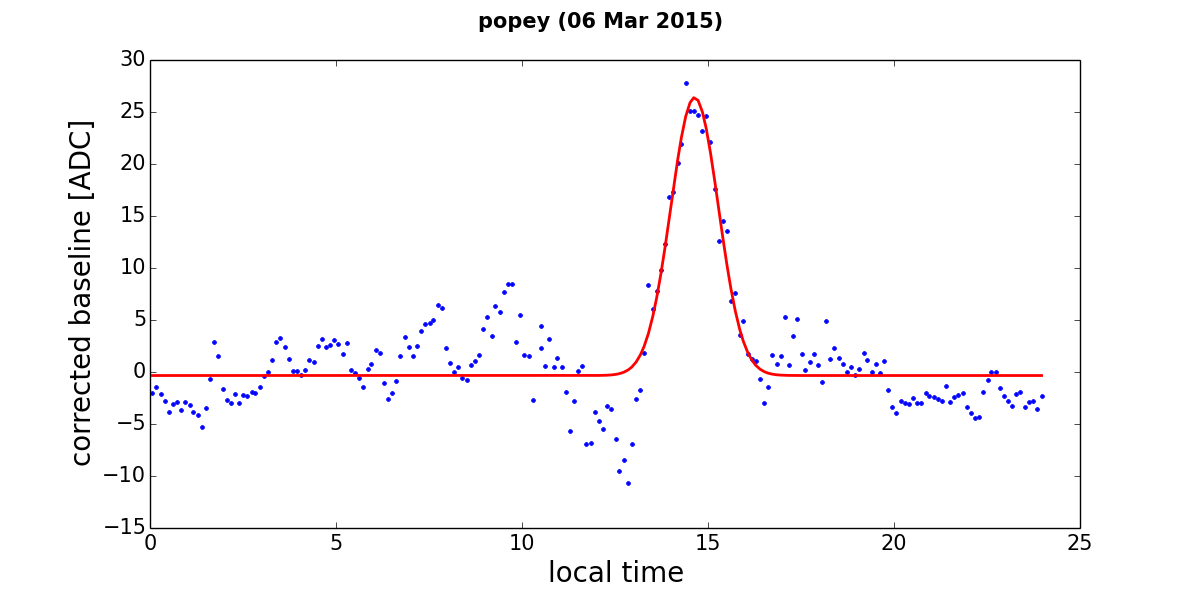
\includegraphics[width=0.49\linewidth]{fitexample.png}}
  \subfigure{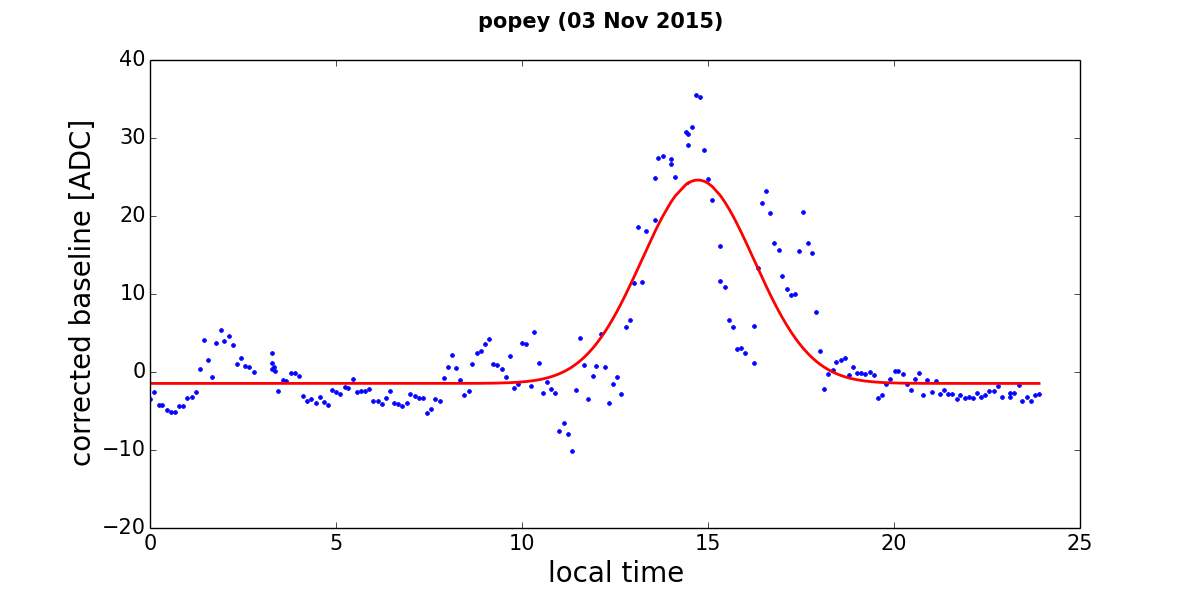
\includegraphics[width=0.49\linewidth]{badfitexample3.png}}
  \caption{Left: good fit example. Right: bad fit}
 \label{fig:examplefit}
\end{figure}
The formula used to retrieve the system temperature is:
\begin{equation}
  \rm
  T_{sys} (F_{sun}, A_{eff}, \Delta P) = \frac{\frac{1}{2} F_{sun} A_{eff}}{10^{\frac{\Delta P}{10}} -1 }
\label{eq:tsys}
\end{equation}
Where $\rm  F_{sun}$ is  the sun flux  measured by  other observatory,
$\rm A_{eff}$ is the effective area in the sun's direction, $\Delta P$
is the power difference in dB (with 1dB = 50 ADC count) and the factor
$\rm \frac{1}{2}$ is  the polarization factor. 

\subsection{Temperature measurement uncertainties}
From the  equation~\ref{eq:tsys}, we can compute  the uncertainties on
$\rm T_{sys}$:
\begin{equation}
  \rm       \sigma_{T_{sys}}^2      =      \frac{T_{sys}^2}{F_{sun}^2}
  \sigma_{F_{sun}}^2  + \frac{T_{sys}^2}{A_{eff}^2} \sigma_{A_{eff}}^2
  +   T_{sys}^2   \bigg(\frac{   \frac{\ln(10)}{10}   10^{\frac{\Delta
        P}{10}}}{10^{\frac{\Delta P}{10}}  - 1}\bigg)^2 \sigma_{\Delta
    P}^2
\end{equation}

\subsubsection{Sun flux uncertainties}
The  sun  flux  at  \unit[3.8]{GHz}  is  based  on  measured  data  at
\unit[2.8]{GHz}     and    the    parameterization     described    in
section~\ref{sec:expectedsignal}. We can  compare our results with the
Nobeyama  observatory data,  which collects  data on  the sun  flux at
\unit[2 and  4]{GHz} (we don't use  their data yet  because they don't
release  them   on  the  web).    The  figure~\ref{fig:sunflux}  shows
different fluxes:

\begin{figure}[!ht]
 \centering
 \hspace*{-3ex}
 \subfigure{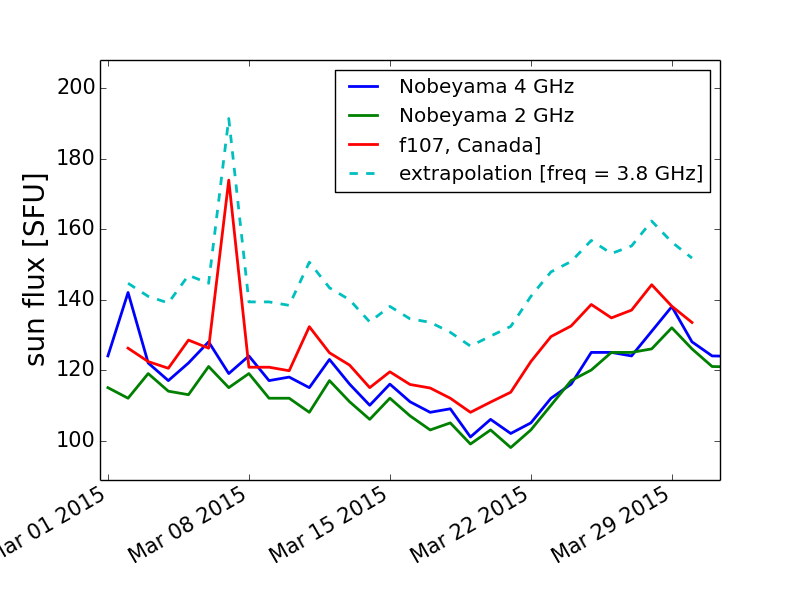
\includegraphics[width=0.49\linewidth]{sunfluxmarch.png}}
 \subfigure{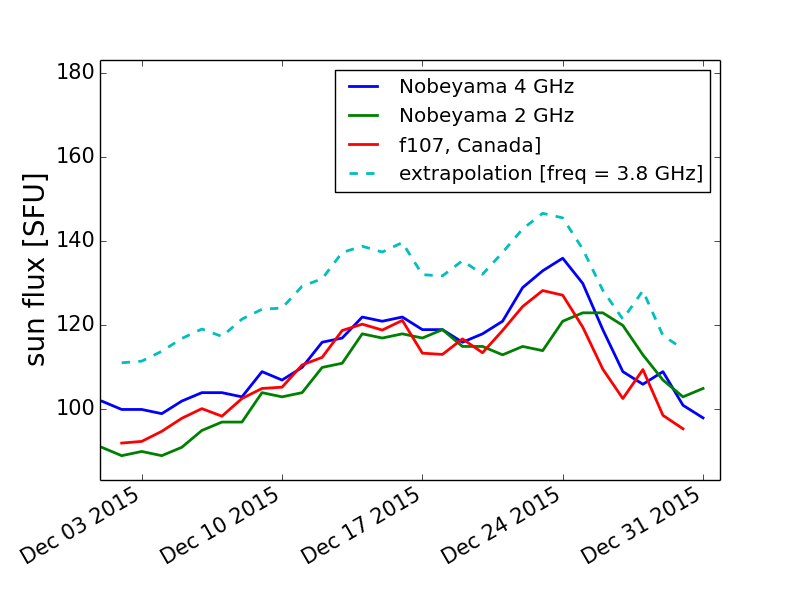
\includegraphics[width=0.49\linewidth]{sunfluxdec.png}}
%% \subfigure{\includegraphics[width=0.49\linewidth]{sunexpected.png}}
 \caption{sun flux for at different frequencies}
%%    Simulated  baseline  increase for  three  antennas  during the  sun
%%    passage.}
 \label{fig:sunflux}
\end{figure}
The value reported on the plots for the Nobeyama observatory are taken
from what is  displayed on their daily curves. I  don't really know if
this is an  average or the minimum value.  In any  case, the values at
\unit[2 and  4]{GHz} are lower than  what is measured  at the Canadian
site~\cite{sundata,  sundata2} by around  20\%. Since  I am  still not
sure of the meaning of the value for the Nobeyama data, I will account
for   an  uncertainty   of   20\%  in   the  temperature   calculation
(\textbf{this has to be improved either by taking the data of Nobeyama
  or by determining a precise uncertainty.}). 20\% corresponds also to
the precision given for the used parameterization~\cite{sunparam}.

\subsubsection{Effective area uncertainties}
Our measurement contains  an uncertainty on the effective  area, be it
because  of the  pointing direction  or our  limited knowledge  of the
gain.  We  only account  the possible shift  in zenith angle,  since a
shift in azimuth  would mainly affect the time  of maximum and slighly
the  amplitude of  the  signal.   We estimate  the  possible shift  in
pointing to  2$\rm ^{\circ}$.  The  resulting uncertainty on  the gain
depends   on   the   zenith   angle   at   the   sun   maximum.    The
Figure~\ref{fig:aeffuncert}  (left) shows  the antenna  effective area
and a  Gaussian fit as a  function of the zenith  angle. The resulting
uncertainties  on  the  effective   area  is  based  of  the  Gaussian
parameters   and    its   angle    dependence   is   shown    on   the
Figure~\ref{fig:aeffuncert} (right).

\begin{figure}[!ht]
 \centering
 \hspace*{-3ex}
 \subfigure{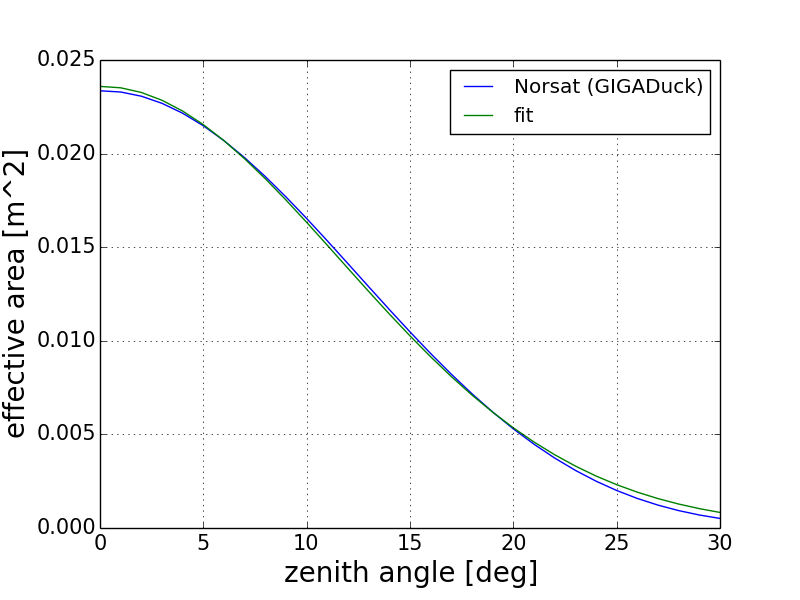
\includegraphics[width=0.49\linewidth]{aeff.png}}
 \subfigure{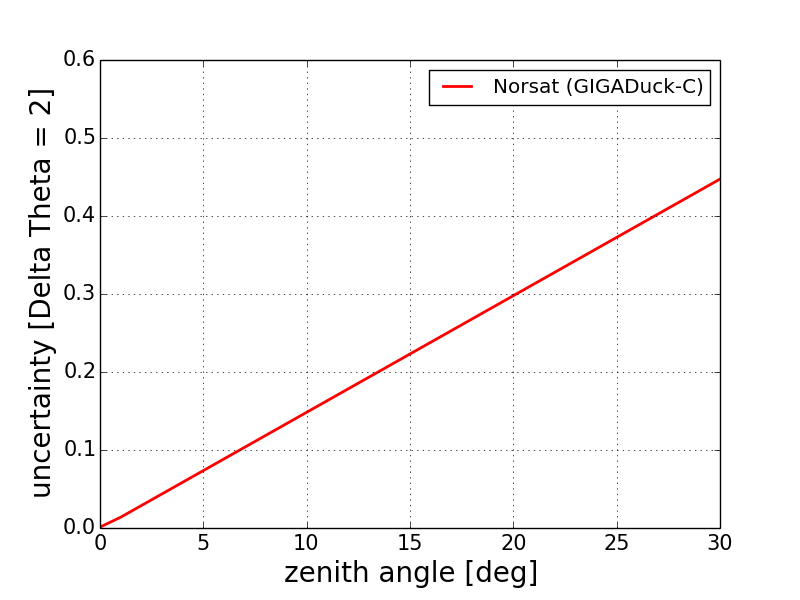
\includegraphics[width=0.49\linewidth]{sigmaaeff.png}}
 \caption{Effective  area of  the AInfo  antenna from  HFSS simulation
   (blue), Gaussian  fit (green).  Right: relative uncertainty  on the
   effective area}
 \label{fig:aeffuncert}
\end{figure}
We perform the  temperature measurement only during the  months when a
significant signal  from the  sun is expected,  that means when  it is
high in the  sky. The zenith angle at which the  sun signal is maximum
(in the  simulation) is shown in  the figure~\ref{fig:zenithofmax} for
three  antenna: Vieira  the central  detector  that points  up to  the
zenith,  Chape and  Orteguina (see  figure~\ref{fig:sunsim}  for their
field of view).
\begin{figure}[!ht]
 \centering
 \hspace*{-3ex}
 \subfigure{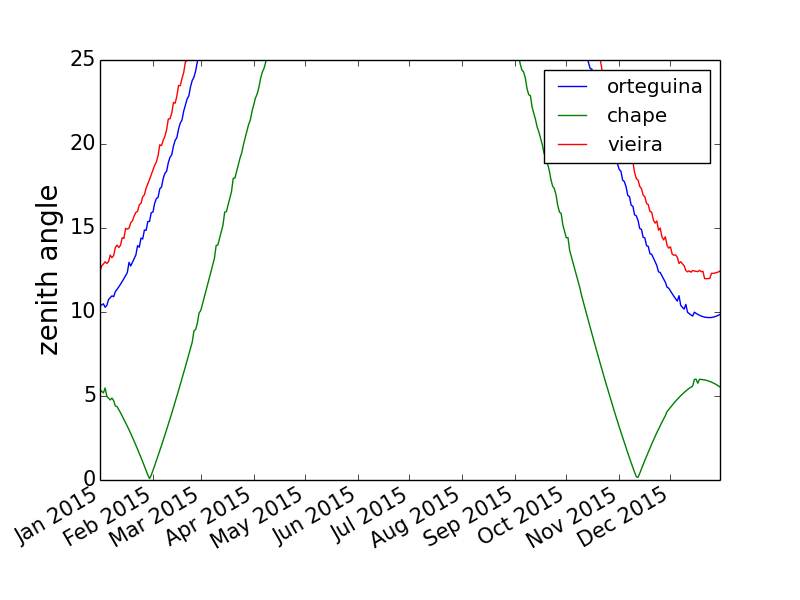
\includegraphics[width=0.49\linewidth]{zenithofmax.png}}
 \caption{Zenith angle when the sun signal is maximum as a function of
   the date}
 \label{fig:zenithofmax}
\end{figure}
The angle at  which the sun is observed when the  signal is maximum is
below  \unit[10]{$\rm  ^{\circ}$} for  Chape  but  around \unit[15  to
  20]{$\rm  ^{\circ}$}   in  March  for  Vieira   or  Orteguina.  This
translates to an uncertainty that can reach up to 40\%.


\subsubsection{Uncertainty on $\rm \Delta P$}
The uncertainty  on the  measured power induced  by the sun  flux $\rm
\Delta P$ comes from our ability to measure a variation of baseline on
an hour time scale.  The process to estimate this variation, summed up
in section~\ref{sec:tempmeas}, is based on  a fit of the sun bump with
a  Gaussian   function  and  the   background  with  a   second  order
polynominals.   There  aren't   actually  any  justification  for  the
background fit. To estimate the error on the $\rm \Delta ADC$ we make,
we  change the fitting  method and  see how  the results  change.  The
figure~\ref{fig:fits}  shows the  results  of $\rm  \Delta  ADC$ as  a
function  of  the date  when  the baseline  is  either  fitted with  a
constant  and a  Gaussian  or with  a  second order  polynomial and  a
constant, on  the right side  is shown the corresponding  histogram of
the difference of the two methods.
